\documentclass[11pt]{article}
\usepackage[utf8]{inputenc}
\usepackage[T1]{fontenc}
\usepackage{amsmath,amssymb,amsthm}
\usepackage{booktabs}
\usepackage{graphicx}
\usepackage[margin=2.7cm]{geometry}
\usepackage{hyperref}
\usepackage{tikz}
\usetikzlibrary{positioning,arrows.meta,calc}
\tikzset{
  ax/.style={draw=blue!60!black, fill=blue!12, rounded corners=2pt, font=\scriptsize, inner sep=3pt, minimum height=5.5mm},
  th/.style={draw=blue!60!black, fill=blue!6, rounded corners=2pt, font=\scriptsize, inner sep=3pt, minimum height=5.5mm},
  goal/.style={draw=green!50!black, fill=green!14, rounded corners=3pt, font=\scriptsize\bfseries, inner sep=3.5pt},
  open/.style={draw, dashed, rounded corners=2pt, font=\scriptsize, inner sep=3pt},
  fl/.style={-{Stealth[length=2mm]}, gray!70},
  gl/.style={-{Stealth[length=2.2mm]}, green!50!black, thick},
}

% ============================================================================
% REGLE D'OR (PLAN.md) : chaque phrase adossee a un objet du depot.
% Les commentaires %% ANCRE: pointent la preuve de chaque section.
% ============================================================================

\newtheorem{definition}{Definition}
\newtheorem{proposition}{Proposition}
\theoremstyle{remark}\newtheorem{example}{Example}

\title{Failure as a Theorem:\\
Certified Error Objects, Fidelity Auditing, and the Instrumented Last Mile\\
in an LCF Kernel for Bourbaki's Theory of Sets}

\author{Karl [full name]\thanks{ISEP Paris. Contact: [email]. Code and certified
corpus: [repository URL and tagged commit hash at submission time].}}

\date{Preprint --- August 2026}

\begin{document}
\maketitle

\begin{abstract}
Proof assistants certify success: a theorem either checks or it does not. We present a
system in which \emph{failure} is certified with the same rigor. Working in an LCF-style
kernel implemented directly over Bourbaki's own formal system --- the $\tau$ operator
and its abbreviated assemblies, a formalism no prior mechanization inhabits --- we
develop (i) \emph{certified
failure objects}: every dead end carries a kernel-checked certificate (e.g.\ a derivation
of absurdity from a residual hypothesis) and a \emph{computed} blast radius; (ii) an
operational trichotomy classifying every open hypothesis as dischargeable, refutable, or
independent --- the first two verdicts kernel objects, the third a default whose epistemic
status we state explicitly; (iii) \emph{debt measurement}: a theorem
advertised as hypothesis-free is measured to consume 53 axioms of ad-hoc theories
invisible to its statement, motivating a sound accounting of what a derivation actually
assumes; and (iv) \emph{mechanized fidelity auditing} against the source text at
page granularity, under which two axiom transcription defects were detected by
\emph{deriving a contradiction}, repaired by restoring the book's form, and proven fixed
by the impossibility of re-deriving it. A Weisfeiler-Leman similarity scan reduces the
detection of one such incoherence from a 95-minute two-agent investigation to a
query of a few seconds.
We report an instrumented week of operation --- three axiom defects found and repaired,
a vacuous theorem revoked and later rehabilitated by discharge, a 3{,}909-test suite ---
and argue that the resulting corpus of certified failures, unavailable from any existing
proof corpus, is the missing training substrate for AI systems intended to \emph{create}
theories rather than merely search for proofs.
\end{abstract}

%% ============================================================================
\section{Introduction}
%% ANCRE: PLAN.md table des revendications C1-C8 ; chiffres CAMPAGNE_DEMOS.md
%% ============================================================================

Proof assistants are engines of certainty: a theorem checks or it does not, and
libraries accumulate the successes. Everything else --- the failed attempts, the
routes that dead-ended, the hypothesis that turned out refutable, the axiom that was
mistranscribed from the book --- is discarded, surviving at best as commit messages
and folklore. Early instrumentation work showed this discarded material can be
captured~\cite{ringer2020replica}, and the current generation of proving agents
consumes failures as training negatives or repair prompts~\cite{april2026,
goedelarchitect2026}. But in every system we know, the failure itself remains an
\emph{unverified} artifact: a compiler message, a model's own diagnosis, a judged
trajectory. Nothing guarantees that the recorded wall was real, that its declared
cause is the actual cause, or that the search it forbids is actually hopeless.

This paper takes the opposite stance: \textbf{failure can be certified with the same
rigor as success}. In our system a dead end is an object carrying a kernel-checked
certificate --- for instance a derivation of absurdity from the residual hypothesis
that killed the route --- together with a \emph{computed} scope stating exactly which
goals it condemns. An infidelity to the source text is not an estimated alignment
score but a derived contradiction. What a theorem silently assumes is not read off
its hypothesis count but measured over its derivation. And the corpus of such objects
demonstrably steers subsequent search: routes certified dead are never paid for twice,
and a revoked theorem, kept with its certificate, can later be rehabilitated
unchanged when its theory is repaired.

The setting sharpens the experiment. We work in an LCF-style kernel implemented over
Bourbaki's \emph{own} formal system --- the $\tau$-operator, its abbreviated
assemblies, and the body of criteria Bourbaki \emph{proves} about demonstrations
instead of positing as rules --- a formalism that, to our knowledge, no prior
mechanization inhabits (Section~\ref{sec:background}). What the kernel implements is
Bourbaki's notion of a \emph{theory}: any name carrying a finite set of explicit
axioms runs through it unchanged, and the corpus mints sixty of them --- which is
precisely why a theorem can quietly consume axioms its statement never mentions.
The oracle is exact, so every
concept of the framework has a decidable or derivable meaning; and the corpus is
small enough to audit completely yet rich enough that, in one instrumented week, the
framework found and repaired three axiom transcription defects (two by deriving a
contradiction), dissolved three phantom walls (of the nine its corpus records),
revoked one vacuous theorem and later
rehabilitated it by discharge, exposed 53 axioms of invisible debt behind a
``hypothesis-free'' theorem, and ended with the full 3{,}909-test suite green
(Section~\ref{sec:casestudy}). This is deliberately the \emph{last mile} of
formalization: the gap between a corpus that merely builds and one that is faithful to
its source, honest about its debts, and instrumented about its failures --- and it is
that instrumented mile, not any single theorem, that this paper measures.

\paragraph{Contributions.}
\begin{enumerate}
  \item The first mechanization, to our knowledge, of Bourbaki's own formalism:
        $\tau$, assemblies and the C1--C62 criteria, as a live, tested corpus
        (Section~\ref{sec:background}).
  \item Certified failure objects with computed scope, and the E1--E7 taxonomy,
        every class instantiated by a real, measured case
        (Section~\ref{sec:certified-failure}).
  \item Debt measurement $Ax(D)$, the axioms a derivation $D$ actually
        consumes --- with the measured gap between declared
        hypotheses and consumed axioms --- and an operational trichotomy of open
        hypotheses whose third branch (independence) we found nowhere else,
        including a negative result on its tempting syntactic shortcut
        (Section~\ref{sec:certified-failure}).
  \item Mechanized fidelity: infidelity as a \emph{derived} verdict against a
        pre-existing printed source, two defects detected and repaired this way, the
        healing itself proved, and the measured cost --- two statements that were
        provable only through the inconsistency (Section~\ref{sec:fidelity}).
  \item A training-free vector detector for twin axioms, calibrated on pairs of
        known status, and the instance-traced returns of the corpus-guided loop
        (Section~\ref{sec:vectors}).
\end{enumerate}

Section~\ref{sec:related} positions each contribution against a systematic,
adversarially-conducted related-work sweep; Section~\ref{sec:limitations} states
what a single-operator, exact-oracle study can and cannot claim.

%% ============================================================================
\section{Background: Bourbaki's Formal System and the Kernel}
%% ANCRE: rapport/ ; theorie_ensembles.py docstring (MemoryError de A1) ;
%% Mathias 4.5e12 ; Grimm/Gaia (sources/grimm_gaia/)
%% ============================================================================
\label{sec:background}

\subsection{A formalism nobody inhabits}
In \emph{Th\'eorie des ensembles}, quantifiers do not exist as primitives. They are
\emph{abbreviations} built from Hilbert's choice operator. Write $R$ for a relation,
$x$ for a letter, and $A$ for an \emph{assembly}: a finite sequence of signs --- the
four logical signs $\square$, $\tau$, $\vee$, $\neg$, the letters, and the specific
signs of the theory --- of which certain pairs are joined by \emph{links}
(E~I.14, ll.~11--16). Then
\[ (\exists x)R := (\tau_x(R) \mid x)\,R , \]
where $(A \mid x)\,R$ is Bourbaki's notation for the assembly obtained by substituting
$A$ for every occurrence of the letter $x$ in $R$ --- written $R[A/x]$ elsewhere.
Since $\tau_x(R)$ itself contains a full copy of $R$, unfolding a quantifier copies the
formula into itself; nested quantifiers grow multiplicatively per level.
The consequences are famous: fully expanded into primitive signs, Bourbaki's numeral
$1$ occupies $4.5 \times 10^{12}$ symbols (Mathias), about $2.4 \times 10^{54}$ in the
1970 edition (Solovay). The links carry the second difficulty: each ties an occurrence
of $\square$ --- which marks the position a bound variable used to occupy --- to the
$\tau$ that binds it. An assembly is therefore a graph, not a string and not a tree,
and has no native syntax in any proof assistant. Finally, since the bound variable
disappears
into the links, the system has no $\alpha$-conversion: substitution is trivial by
design, which is precisely the property Grimm cites when explaining why Gaia
formalizes the \emph{content} of Bourbaki over Coq's own logic and treats Chapter~I
--- assemblies, $\tau$, the deduction criteria --- as description only. To our
knowledge (Section~\ref{sec:related}), no prior mechanization inhabits the formalism
itself; it is, however, exactly where Bourbaki's metatheory lives: the criteria are
theorems \emph{about} theories --- among them C62, the licence for every definition
by recursion, which the corpus leans on throughout.

\subsection{The kernel: inhabiting it anyway}
The kernel is written in pure Python, in the LCF style.

\begin{definition}[Abbreviated terms and relations]\label{def:langage}
The sets $\mathcal{T}$ of \emph{terms} and $\mathcal{R}$ of \emph{relations} are
defined by mutual induction, exactly as the kernel represents them:
\begin{align*}
  T &::= x \;\mid\; s(T_1,\dots,T_n) \;\mid\; \tau_x(R)
     &&\text{(letter, specific sign, choice)}\\
  R &::= (T = U) \;\mid\; (T \in U) \;\mid\; \neg R \;\mid\; (R \vee S)
        \;\mid\; (\exists x)R
     &&\text{(the five relation-formers)}
\end{align*}
where $x$ ranges over letters, $s$ over the specific signs of the theory, and
$T, U \in \mathcal{T}$, $R, S \in \mathcal{R}$. These eight constructors are the only
ones: $\forall$, $\wedge$, $\Rightarrow$ and $\Leftrightarrow$ are abbreviations built
from them, in Bourbaki's sense and in the code alike.
\end{definition}

\begin{definition}[Theorem object]\label{def:theoreme}
Write $\mathcal{P}_{\mathrm{fin}}(\mathcal{R})$ for the set of finite subsets of
$\mathcal{R}$, and let $\mathcal{J}$ be the set of justification labels: the name of
the kernel rule applied and, for the axiom rule, the theory it was drawn from ---
which is what makes the debt of Section~\ref{sec:certified-failure} observable at all.
A \emph{theorem} is an element
\[ \theta \;\in\; \mathcal{P}_{\mathrm{fin}}(\mathcal{R}) \times
   \mathcal{R} \times \mathcal{J} . \]
Its three projections are written $H$, $C$ and $j$:
\begin{itemize}\itemsep2pt
  \item $H(\theta) \subseteq \mathcal{R}$, finite --- the \emph{hypotheses} $\theta$
        still depends on;
  \item $C(\theta) \in \mathcal{R}$ --- the \emph{conclusion} $\theta$ asserts;
  \item $j(\theta) \in \mathcal{J}$ --- the \emph{justification}, that is, the rule
        that produced $\theta$.
\end{itemize}
The theorem is \emph{closed} when
$H(\theta) = \emptyset$. Equality is on the first two projections only,
\[ \theta = \theta' \iff H(\theta) = H(\theta') \ \text{ and } \ C(\theta) = C(\theta') , \]
so the justification records how a theorem was obtained, not what it asserts.
\end{definition}


\begin{example}[A theorem, end to end]
Take the relation $x \in E$: by Definition~\ref{def:langage} it is built by the
$\in$ former from two letters. Assuming it gives the theorem
\[ \theta_1 : \quad H(\theta_1) = \{\, x \in E \,\}, \qquad
   C(\theta_1) = (x \in E), \qquad j(\theta_1) = \text{hypothesis}, \]
which is \emph{not} closed --- it asserts its conclusion only under its own
assumption. Discharging that assumption with the deduction rule gives
\[ \theta_2 : \quad H(\theta_2) = \emptyset, \qquad
   C(\theta_2) = \bigl((x \in E) \Rightarrow (x \in E)\bigr), \qquad
   j(\theta_2) = \text{deduction}, \]
which is closed. Nothing was proved about $E$ along the way: what the second object
records is that the hypothesis has moved from the left of the turnstile into the
conclusion. That move is the whole of \emph{discharge}, and Section~\ref{sec:certified-failure}
turns on the fact that it is the only thing a hypothesis count reflects.
\end{example}

Theorem objects are opaque: they are constructible only through the kernel's rules,
and no other code in the corpus may fabricate one.

Bourbaki's own demonstrations use a \emph{single} rule: a demonstration is a sequence
in which every relation is an axiom --- explicit, or an instance of a scheme --- or is
detached from two earlier ones, $R$ and $R \Rightarrow S$ (E~I.22, ll.~16--25).
Everything else he needs, including the deduction criterion and generalization, he
establishes as \emph{criteria}: metatheorems about demonstrations, proved once.

Our kernel departs from this on two counts, and both enlarge the trusted base
deliberately. It takes the deduction criterion and generalization as \emph{primitive}
rules rather than re-deriving them at each use --- the code marks them as trusted
primitives, not derived --- and it carries the hypothesis set $H$ inside the theorem
object, where Bourbaki would instead move to a stronger theory. Beyond these, the rules
are detachment, the schemes S1--S7, and explicit axioms.

The schemes are not a flat list, and set theory is not the whole story. Bourbaki builds
theories in a tower, each level adding its own \emph{implicit} axioms: S1--S4 belong to
the \emph{logical} theories (E~I.25), S5 to the \emph{quantified} theories (E~I.33),
S6 and S7 to the \emph{egalitarian} theories (E~I.38). Set theory is then the
egalitarian theory that adds the membership sign together with its own \emph{explicit}
axioms, and the corpus is laid out along that tower rather than around its top floor.
This is why the invariant we check counts 22 \emph{explicit} axioms: everything below
is inherited as schemes, and a theorem may consume any of it without the count moving
--- the gap that Section~\ref{sec:certified-failure} turns into a measurement.

The criteria are stratified the same way, and they are not kernel rules. Each
is a metatheorem about demonstrations \emph{in a theory}, proved at the level where it
first becomes statable --- most of them among the logical theories, generalization
(C27) among the quantified ones, and the later ones only once set theory is available.
Of the whole series the kernel takes exactly three as primitives: detachment C1,
deduction C14, generalization C27. The others are derived, and a good many of them are
derived inside the corpus itself, which is what makes ``we inhabit C1--C62'' a claim
about a tested library rather than about a design intention.

Two design decisions make the formalism workable:

\emph{Abbreviated trees, expansion as justification.} Building the axiom
$A1$ of extensionality by full $\tau$-expansion exhausts memory --- a
\texttt{MemoryError} reproducible
on demand and journaled, faithful to Bourbaki's own remark on the practical necessity of
abbreviations. The kernel therefore represents $\forall/\exists$ as first-order abbreviators
at tree level; the $\tau$-expansion remains the \emph{justification} of the rules,
not the runtime representation.

What is left unexpanded is the \emph{quantifier abbreviation}, not $\tau$. The choice
operator is a primitive term-former of the kernel, governed by Bourbaki's own scheme
S7 (E~I.38, ll.~22--24): for any relations $R$ and $S$ and any letter $x$,
\[ (\forall x)(R \Leftrightarrow S) \;\Rightarrow\; \tau_x(R) = \tau_x(S) . \]
The operator is inhabited throughout the corpus. For a graph $f$, that is a set of
ordered pairs,
and any object $x$, the value $f(x)$ \emph{is} the term $\tau_y((x,y) \in f)$
(E~II.13). The term is well formed whatever $f$ and $x$ may be; it denotes what one
expects of a value only when $f$ is functional and $x$ lies in its domain. Keeping
that gap visible rather than hiding it behind a typing discipline is what makes a
proof fail loudly instead of quietly, and Section~\ref{sec:certified-failure} is
largely about what that buys. The projections of a pair, the cardinals, and every
canonical witness we build in place of an appeal to choice are $\tau$-terms in the
same way. This is where the
system departs from assistants that take $\forall/\exists$ as logical primitives and
carry no choice operator in the kernel at all. It is also paid for: because $\exists$
is a primitive node rather than a $\tau$-abbreviation at runtime, a few results proved
at the $\tau$ level --- reflexivity of equality among them --- are transported into the
abbreviated level as trusted primitives. That is the third and last enlargement of the
trusted base, and the code marks each one.

The residual cost is real and measured: cardinal
terms are $\tau$-terms, constructing $\mathbb{N}$-dependent objects costs minutes per
process, printing a cardinal term is never attempted (its expansion is intractable in
practice), and one
instantiation from variables to closed terms takes a formula from 9{,}388 to 86{,}598
characters. This cost is a property of the formalized system, not of the
implementation; it is also, as Section~\ref{sec:vectors} shows, the reason caching
and vectorization matter.

\emph{No $\alpha$-identification.} The kernel does not identify $\alpha$-variants:
two $\alpha$-equivalent formulas are distinct objects, compared by a dedicated
predicate and converted by an explicit certified bridge. This strictness is what
makes drift (Section~\ref{sec:certified-failure}) detectable at all --- and what
makes hard-coded binder names a recurring, measurable trap.

\emph{Dedicated theories.} Beyond the 22 explicit axioms of the reference theory, the
corpus mints small ad-hoc theories: 60 factories at the time of writing, 19 of them
parametric. Each comes from Bourbaki's
scheme of selection, which licenses naming the set of elements of a given set that
satisfy a given relation, and giving that name its own characterizing axiom. The device
is legitimate and unavoidable, and it has one consequence nobody measures --- the
invisible debt of Section~\ref{sec:certified-failure} --- and one genuinely dangerous
corner: theorem objects carry no trace of their theory, so the kernel cannot see that
a free variable of an ad-hoc axiom is a \emph{constant} of that theory when
generalizing.

The corpus at the time of writing: 4{,}099 collected tests re-deriving its theorems at
each run, 2{,}234 notions anchored to the printed book at page granularity, and a
232-event journal of certified failures --- the object of study of this paper.

Its weight is worth stating, because the name of the book invites a wrong picture. The
2{,}181 notions anchored at the time of the campaign reported in
Section~\ref{sec:case-study} distribute over the tower and the chapters it carries as
follows (the corpus has since grown to 2{,}234; the breakdown is a snapshot, not a
running total):

\begin{center}\small
\begin{tabular}{llr}
\toprule
\S I.1 & assemblies, formative constructions & 82 \\
\S I.2 & demonstrations, the criteria, the kernel & 133 \\
\S I.3 & \emph{logical} theories & 5 \\
\S I.4 & \emph{quantified} theories & 32 \\
\S I.5 & \emph{egalitarian} theories & 22 \\
\midrule
Ch.~II & sets proper & 720 \\
Ch.~III & ordered sets, cardinals, integers & 1{,}002 \\
Ch.~IV & structures & 185 \\
\bottomrule
\end{tabular}
\end{center}

Two readings matter here. First, the set-theoretic level is about a third of the
corpus and the largest single part is Chapter~III, while the claim of novelty ---
inhabiting $\tau$, assemblies and the criteria --- concerns Chapter~I:
\emph{Th\'eorie des ensembles} names the book, which erects the whole tower, not one
privileged level. Second, the three theory levels look thin only because the corpus is
filed by \emph{kind} rather than by floor: the criteria proved in the logical theories
are counted under \S I.2 with the rest of the criteria, which is where a reader of the
repository will find them.


%% ============================================================================
\section{Certified Failure: Definitions, Taxonomy, Objects}
%% ANCRE: outils_ia/verite/README.md ; echec.py ; classer_residu.py ; events.jsonl
%% ============================================================================
\label{sec:certified-failure}

Throughout, a \emph{theory} $T = (\mathit{name}, A_T)$ is a name together with a finite
set $A_T \subseteq \mathcal{R}$ of relations, its \emph{explicit} axioms. Its implicit
axioms --- the schemes S1--S7 of the tower of Section~\ref{sec:background} --- are
deliberately absent from the pair: every theory in this corpus stands on the same
egalitarian floor, so the schemes are kernel rules available to all of them rather than
data carried by each. We write $T_0$ for the reference theory, so that $A_{T_0}$ is the
22 explicit axioms of the set-theoretic level; the ad-hoc theories minted by
selection are further $T$'s, usually with a single axiom of their own, and it is their
invisibility to a theorem's statement that the debt below measures. Finally $\theta$ is
a theorem object in the sense of Definition~\ref{def:theoreme}, with projections
$H(\theta)$, $C(\theta)$, $j(\theta)$.

We write $\Gamma \vdash R$, for a finite $\Gamma \subseteq \mathcal{R}$, when the
kernel can construct a theorem $\theta$ with $C(\theta) = R$ and
$H(\theta) \subseteq \Gamma$; $A_T \vdash R$ additionally allows the axioms of $T$ to
enter through the $\mathsf{axiome}$ rule, and $\vdash R$ alone means $\emptyset \vdash R$,
a closed theorem. This is a statement about what the kernel \emph{can build}, so every
$\vdash$ in this paper is witnessed by an object, never asserted.

A \emph{route} to a goal is one attempted derivation of it, and the \emph{residue} of
a route is the set of hypotheses the theorem it reaches still carries --- that is,
$H(\theta)$ for the $\theta$ the route produced. A goal typically has several routes,
and the same hypothesis may be open on one and closed on another; that is why the
verdicts below are stated of a hypothesis \emph{on a route}, not of a hypothesis
outright.

Bourbaki's system has no primitive falsum; we fix the closed witness
$\bot := (\emptyset \in \emptyset)$, since $\vdash \neg(\emptyset \in \emptyset)$ is
closed from the axiom of the empty set.

\subsection{Debt: what a derivation actually assumes}
\begin{definition}[Consumption and debt]
Call a \emph{derivation} $D$ of a theorem $\theta$ the finite sequence of kernel-rule
applications that produced it. One of those rules is
\[ \mathsf{axiome}(T, \alpha) , \qquad T \text{ a theory}, \ \alpha \in A_T , \]
which returns the closed theorem asserting $\alpha$ and refuses any $\alpha$ outside
$A_T$: it is the only way an axiom can enter a derivation, which is what makes the
following observable at all. Let
\[ Ax(D) := \{ (T, \alpha) \mid \text{the rule } \mathsf{axiome}(T,\alpha) \text{ occurs in } D \}. \]
The \emph{debt} of $\theta$ derived by $D$ is
\[ \mathit{Debt}(\theta) := H(\theta) \cup \{ \alpha \mid (T,\alpha) \in Ax(D),\, T \neq T_0 \}, \]
and the \emph{real invariant} is $Ax(D) \subseteq \{T_0\} \times A_{T_0}$.
\end{definition}

Both lines are worth reading in words. The first says that what $\theta$ actually
leans on is what it still assumes, \emph{plus} every axiom its derivation drew from
somewhere other than the reference theory --- and that only the first half of that is
visible in its statement.

The second is the honest form of ``the theory has 22 axioms''. That familiar invariant
is a property of a theory \emph{object}: one counts the axioms of $T_0$ and gets 22,
today and every day, whatever anyone proves. The invariant above is a property of a
\emph{derivation}, and it says something much stronger --- that this particular proof
owed nothing outside the reference theory. A corpus can satisfy the first everywhere
and violate the second constantly, and that gap is what the rest of this section
measures.

A theorem's hypothesis count records only what \emph{discharge} left behind --- the
kernel's deduction rule removes a hypothesis by turning it into an implication, and
what survives that process is $H(\theta)$. It records nothing about what the derivation
had to reach for along the way. The debt does: it keeps the hypotheses and adds every
axiom drawn from a theory other than $T_0$, and nothing in the statement bounds that
addition.

Our measured instance is a theorem of the corpus advertised as ``closed, 0
hypotheses'' --- the well-ordering of $\mathbb{N}$. Its derivation was measured to
apply the $\mathsf{axiome}$ rule \textbf{67 times, 53 of those on ad-hoc theories}.
Both its statement and the global axiom count, which stayed at 22 throughout, were
blind to all 53.

The instrument is an observer placed around the $\mathsf{axiome}$ rule: the kernel is
not modified, and each time the rule is entered the pair $(T, \alpha)$ is recorded.
This makes one failure mode intrinsic and worth stating. Several proof functions in the
corpus are memoized; on a second call within the same process the cached theorem is
returned and its body never runs, so the rule is never entered and the observer sees
an empty $Ax(D)$ for a derivation that does consume axioms. Measured, this undercounts
by up to $62\%$. A measurement is therefore valid only in a fresh process and in first
position --- and the corpus carries a test that \emph{exhibits} this false negative
rather than papering over it.

\subsection{Vacuity, drift, phantom walls}
\begin{definition}[Vacuity] $\theta$ is \emph{vacuous in} a theory $T$, written
$\mathit{Vac}_T(\theta)$, when $A_T \cup H(\theta) \vdash \bot$. Vacuity is thus
relative to $T$: the same theorem can be vacuous in one theory and sound in a
stronger one, which is exactly what rehabilitation exploits below.
\end{definition}
A theorem can be perfectly derived and yet worthless: soundness is a property of the
derivation, vacuity of the model class. Our measured instance: $0! = 1$ (Def.~2 route)
was proved under $\mathcal{H} := (\forall G)(G \in \prod(u,\emptyset) \Rightarrow
\mathrm{Gr}(G))$, and $\{\mathcal{H}\} \vdash \bot$ was then derived --- the theorem was
revoked. Crucially, it was later \emph{rehabilitated unchanged}: after the axiom repair
of Section~\ref{sec:fidelity}, $\mathcal{H}$ became a closed theorem and the identical
proof skeleton re-derived with the hypothesis discharged. A vacuous theorem is not a
wrong theorem; it is a theorem waiting for its theory.

\begin{definition}[Drift]
Let $C^\ast \in \mathcal{R}$ be the \emph{intended conclusion} of $\theta$: the
relation $\theta$ is meant to have, written out from the book's statement in a test
file that shares no code with the module proving $\theta$. Then
\[ \mathit{Drift}(\theta, C^\ast) \iff \theta \text{ builds, is closed, passes its
   tests, and } C(\theta) \neq C^\ast \]
as relations --- syntactic inequality, not failure.
\end{definition}

The independence of $C^\ast$ is the whole point. A test that compares $\theta$'s
conclusion against an expression built by the \emph{same} module compares a thing with
itself: change the module and both sides move together, and the test stays green while
the theorem quietly becomes a different theorem. Drift is thus invisible to the kernel,
since nothing is false, and invisible to any test that is not independently anchored.

Measured instance: after an axiom change, one theorem of the corpus still built and
remained closed while its conclusion grew from 6{,}908 to 8{,}592 characters; its test
asserted only closedness and would have stayed green. Two rules follow, and we apply
them: targets are rebuilt outside the module and compared syntactically, and
hypothesis sets are compared by exact set equality, never by cardinality.

\subsection{The trichotomy of open hypotheses}
\begin{definition}[Trichotomy]
For an open hypothesis $h$ carried by a route over $T$:
$h$ is \emph{dischargeable} iff $A_T \vdash h$;
\emph{refutable} iff $A_T \vdash \neg h$ (then every $\theta$ carrying $h$ is vacuous);
\emph{independent} otherwise --- no amount of proof search will close it, and the only
legal moves change the theory --- as in Figure~\ref{fig:extension}.
\end{definition}

All three classes occurred, measured, within one week: $bo(\le,\mathbb{N})$ ---
declared an ``irreducible residue'' for weeks --- is dischargeable (closed, 0
hypotheses); $\mathcal{H}$ above is refutable; the family-value bridge $X_\iota =
f(\iota)$ is classified independent of $A_{T_0}$. The fourth epistemic state,
\emph{unknown}, is a measurement debt, not a wall: re-classifying it after each
infrastructure fix eliminated nine phantom walls in our corpus.

\begin{proposition}[A negative result]
The syntactic criterion ``some symbol of $h$ is constrained by no axiom of $T_0$'' is
\emph{not} a sufficient test of independence.
\end{proposition}
Counterexample, measured: $\mathit{symboles\_libres}(bo(\le,\mathbb{N})) \neq
\emptyset$, yet the hypothesis is provably closed. The criterion is an \emph{indication}
(a reinterpretation argument is available) and must be applied only after a prover has
failed; applied first, it would have manufactured one more phantom wall.

The asymmetry within the trichotomy is essential.
\emph{Dischargeable} and \emph{refutable} are witnessed by kernel objects;
\emph{independent} is not, and cannot be: it is the \emph{absence} of both witnesses.
The classifier therefore returns \emph{independent} only after a prover has failed
and the free-symbol indication holds --- an ordering of evidence, not a proof.
Independence and \emph{unknown} are distinguished operationally, by the strength of
the prover that failed, never certified. This is the one branch of the trichotomy
whose verdict is defeasible, and the corpus records it as such.

\subsection{Failure objects and their validity conditions}
\begin{definition}[Certified failure]
$\mathit{Echec} = (P, \kappa, c, \mathit{backtrack}, \mathit{scope})$ --- we keep the
repository's French names, $\mathit{Echec}$ (failure) and $\mathit{Mur}$ (wall), to
match the code. Here $P$ is the goal that was being attempted, $\kappa \in
\{E1,\dots,E7\}$ its failure class, $c$ a kernel object certifying that class,
$\mathit{backtrack}$ the stated change that avoids falling into it again, and
$\mathit{scope}$ the \emph{computed} set of goals the failure condemns. $\mathsf{verifier}$ accepts
iff $c$ matches $\kappa$: for $E2$ (vacuity), $C(c) = \bot$ and $H(c) \subseteq$ the
route's residue; for $E5$ (phantom), $c$ is closed and $C(c)$ \emph{is} the declared
residue; etc. A failure whose certificate fails verification is \emph{rejected from the
corpus}.
\end{definition}

\begin{definition}[Wall] $\mathit{Mur} = (\mathit{condition}, \mathit{predicate}, c)$:
while $\mathit{condition}$ is unrepaired, every goal satisfying $\mathit{predicate}$ is
doomed, and $\mathit{predicate}$ \emph{computes} the scope rather than asserting it.
\end{definition}
Measured instance: the refutation witness behind $\mathcal{H}$ hard-codes the empty
index, so the wall's predicate provably reaches only products over a literally empty
index --- H2 (index $I \cup \{j\}$) and H3 (variable index) were \emph{proved out of
reach}, and exactly one file was revoked. Figure~\ref{fig:wall} shows such a wall
in place, with the verdict of each hypothesis it leaves open.

%% ANCRE fig:wall (verifie 2 aout, ev. 98) : frontiere du pas de recurrence
%% {n∈N,H2,H3,HW,HN} = CAMPAGNE_DEMOS l.395-396 (grep asserts) ; HW/HN independantes
%% l.558+681 ; bo = route C62-existence (ev. 9, 61) ; H = route cas-0 (ev. 67) ;
%% mur (n+1)! = ev. 2 (9 hyps succ) + ev. 85 (pont de domaine, cul-de-sac n-1).
%% La legende DIT l'agregation : ce n'est PAS un instantane unique du journal.
\begin{figure}[t]\centering
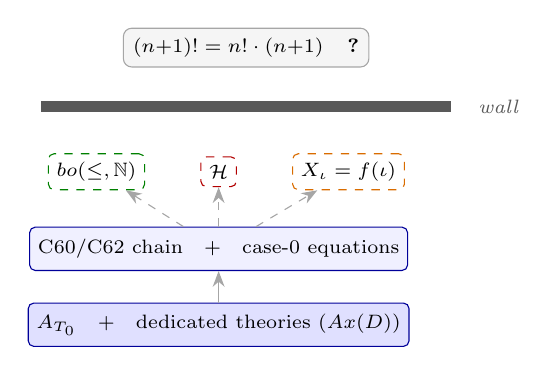
\begin{tikzpicture}[node distance=5mm and 7mm]
\node[goal, draw=gray!70, fill=gray!8] (P) {$(n{+}1)! = n!\cdot(n{+}1)$ \; \textbf{?}};
\node[below=3mm of P, font=\scriptsize\itshape, gray!70!black] (mur)
  {\rule{52mm}{1.4mm}};
\node[right=1mm of mur, font=\scriptsize\itshape, gray!70!black] {wall};
\node[open, draw=green!50!black, below=4mm of mur, xshift=-19mm] (bo)
  {$bo(\le,\mathbb{N})$};
\node[open, draw=red!70!black, right=of bo] (hg) {$\mathcal{H}$};
\node[open, draw=orange!85!black, right=of hg] (hw) {$X_\iota = f(\iota)$};
\node[th, below=5mm of hg] (chain) {C60/C62 chain \; + \; case-0 equations};
\node[ax, below=4mm of chain] (axs)
  {$A_{T_0}$ \; + \; dedicated theories $(Ax(D))$};
\draw[fl] (axs) -- (chain);
\draw[fl, dashed] (chain) -- (bo);
\draw[fl, dashed] (chain) -- (hg);
\draw[fl, dashed] (chain) -- (hw);
\end{tikzpicture}
\caption{A real wall: the factorial front's last open equation. Solid boxes are
kernel objects, dashed boxes are the hypotheses the derivation chain leaves
\emph{open}, and the bar is the wall standing between them and the goal. Box colour
is the trichotomy verdict of Table~\ref{tab:frontier}.}
\label{fig:wall}
\end{figure}

\begin{table}[t]\centering\footnotesize
\begin{tabular}{llll}
\toprule
open hypothesis & met on & verdict & outcome \\
\midrule
$bo(\le,\mathbb{N})$ & the C62-existence route
  & \textcolor{green!50!black}{dischargeable}
  & declared irreducible, later proved closed \\
$\mathcal{H}$ & the case-$0$ route
  & \textcolor{red!70!black}{refutable}
  & source of the vacuity; theorem revoked \\
$H_2$, $H_3$ & the recursion step
  & \textcolor{green!50!black}{dischargeable}
  & fell with the axiom repair of Sec.~\ref{sec:fidelity} \\
$H_W$, $H_N$ & the recursion step
  & \textcolor{orange!85!black}{independent}
  & no search closes them; only the theory can change \\
\bottomrule
\end{tabular}
\caption{The front's frontier, aggregated across its routes rather than taken from
a single journal snapshot. The recursion step's measured residue was
$\{n{\in}\mathbb{N}, H_2, H_3, H_W, H_N\}$, and the trichotomy split it. Each row is
a measured case, and each failure is recorded as a certified object.}
\label{tab:frontier}
\end{table}

\begin{table}[h]\centering\footnotesize
\setlength{\tabcolsep}{4.5pt}
\begin{tabular}{lllp{4.3cm}}
\toprule
class & definition & valid certificate & measured instance \\
\midrule
E1 drift & $C \neq C^\ast$ & syntactic comparison & $\mathit{membre\_but}$ (6{,}908 $\to$ 8{,}592 chars) \\
E2 vacuity & $\{h\} \vdash \bot$ & theorem with $C = \bot$ & $\mathcal{H}$ / revoked $0! = 1$ \\
E3 dead end & no continuation closes & prunes extensions & the ``$n{-}1$'' route (opaque difference term), ev.~84--85 \\
E4 debt & $Ax(D) \not\subseteq \{T_0\}{\times}A_{T_0}$ & fresh-process measure & $n\_bien\_ordonne$: 53 foreign axioms \\
E5 phantom & residue already provable & closed theorem $=$ residue & $bo(\le,\mathbb{N})$, 9 cases total \\
E6 infidelity & $A_{T_0} \cup \Phi \vdash \bot$ & closed derivation $+$ source anchor & two axiom defects (Sec.~\ref{sec:fidelity}) \\
E7 measurement & the probe lied & counter-measurement & name-guessing probe (false negative) \\
\bottomrule
\end{tabular}
\caption{The failure taxonomy. Every class is instantiated by a real, kernel-checked
case from the instrumented week.}
\end{table}

%% ============================================================================
\section{Mechanized Fidelity: When the Corpus Refutes the Book}
%% ANCRE: CAMPAGNE_DEMOS (26-27 juil + 1 aout) ; derivation D1 ; @livre 2033 notions
%% ============================================================================
\label{sec:fidelity}
\subsection{The anchoring discipline and the infidelity verdict}
Every formalized notion carries a machine-readable anchor
\texttt{@livre Ch.X \S{}s.ss Type.n | E X.pp L.a-b | PDF p.n} tying it to the printed
source (2{,}234 anchored notions at the time of writing). The anchor has two fields of
different reliability, and we separate them because we measured them.

\paragraph{The page anchor is sound; the line interval is not uniformly so.} The page
field is what carries the coverage results below: zero non-conforming anchors, and five
parts of the book reported complete over their intervals. The line interval is weaker,
and we discovered this by auditing our own anchors against the book. On page E~II.22 ---
36 printed lines, counted by hand --- Definition~1 stands at lines 15--18 and
Definition~2 at 27--30, while their anchors read \texttt{L.31-36} and \texttt{L.49-53};
the second exceeds the page. Line 53 of our \LaTeX{} \emph{transcription} of that page,
however, is exactly the header of Definition~2: those two anchors index the
transcription, not the book. On page E~II.7 the opposite holds --- the anchor tracks the
printed line with a small offset and does not match the transcription at all. At least
two conventions coexist in the corpus.

Measured over the 1{,}992 anchors carrying a line interval: \textbf{12.2\% end beyond
line 36}, which is about a full page of this edition, so they cannot be printed-line
references; the maximum is 63. The bulk of the distribution has the shape of a printed
page, with a tail that does not.

We therefore claim traceability \emph{at page granularity}, which is what the coverage
instruments actually consume, and we report the intra-page line intervals as a
\emph{heuristic} for locating unformalized material rather than as a certified measure.
This is a weaker claim than the one this paper made in draft, and the reason to record
it here is that it is the paper's own thesis turned on the paper: no test in a
kernel-verified repository catches an anchor that misdescribes the book, and ours went
unexamined until we opened the pages. Let
$\Phi$ be the transcription of the book's numbered statements. Fidelity itself ---
``$\varphi(b)$ \emph{means} $b$'', for a statement $b$ of the book and its
formalization $\varphi(b)$ --- relates text to formulas and is not formalizable;
its negation is:
\[
\mathit{Infid} \iff A_{T_0} \cup \Phi \vdash \bot .
\]
$\mathit{Infid}$ is semi-decidable: one can always \emph{find} an infidelity, never
certify its absence --- which is why our audit is a standing process rather than a
coverage percentage. Two consequences of the discipline are mechanizable for free:
two anchors citing the same sentence at different lines expose an error by mere
comparison (two real cases found and fixed); and a copied line number propagates ---
one wrong value was found replicated verbatim across five sites.

Recent project-scale autoformalization also records span-level provenance; the state
of the art, M2F~\cite{m2f2026}, then enforces statement faithfulness ``by a
provenance-linked \emph{manual audit}'' (p.~8). Our departure is precisely there: the
infidelity verdict is \emph{derived}. Both defects below were established by proving a
contradiction in the kernel, and both repairs were proved effective by the
impossibility of re-deriving it.

A third defect, found the same week, seeded the method. The intersection axiom had
been transcribed from the book's \emph{Summary of Results} (E~R.19), whose universe
of families of \emph{subsets} makes $\bigcap_{\emptyset} = E$ legitimate, rather than
from E~II.22, whose Definition~2 requires $I \neq \emptyset$ (and whose footnote warns
that the unrestricted intersection is not collectivizing). The reference theory
itself was therefore inconsistent. The defect was localized by machine
proof, its blast radius computed at 34 sites, and repaired by restoring the selection
form, holding the axiom count at 22; the incident was closed, suite green, before any
debt measurement reported in this paper was taken. The two cases below were then
found \emph{by} the discipline that this first incident instituted.

\subsection{Case 1: an axiom lost a conjunct}
The product-of-a-family axiom had lost the book's bound on the graphs it admits: for a
family $(X_\iota)_{\iota \in I}$ of sets indexed by $I$, a member $F$ of the product
must satisfy $F \subset I \times \bigcup_{\iota \in I} X_\iota$ (its sibling, the
exponentiation axiom, had kept its own). The corpus then proved, at \emph{zero}
hypotheses and for any family $u$, both
$\{\emptyset\} \in \prod(u,\emptyset)$ and
$\neg(\prod(u,\emptyset) = \{\emptyset\})$ --- while E~II.32 states that the empty
product has exactly one element. The corpus refuted the book. Soundness was never at
issue: the kernel faithfully derived from the axiom it was given; the axiom was not
the book's. The repair restored the conjunct \emph{in head position} (an empirical
choice: 18 broken tests against 33 for tail position), kept the axiom count at 22
(replacement, not addition), and paid immediately: two hypotheses carried for weeks
became theorems, and the vacuous $0! = 1$ of
Section~\ref{sec:certified-failure} was rehabilitated by discharge.
Figure~\ref{fig:proofgraph} shows that rehabilitated derivation, with
the branch the defect had blocked marked in green.

\begin{figure}[t]\centering
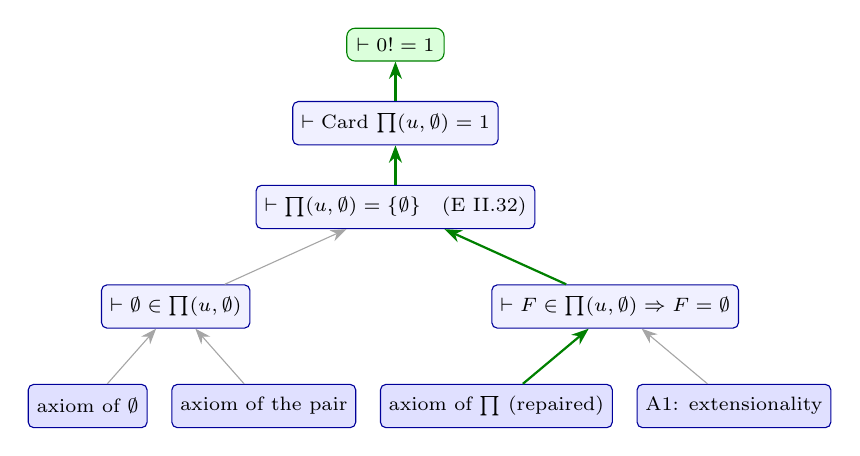
\begin{tikzpicture}[node distance=4mm and 3mm]
\node[ax] (vide) {axiom of $\emptyset$};
\node[ax, right=of vide] (paire) {axiom of the pair};
\node[ax, right=of paire] (prod) {axiom of $\prod$ (repaired)};
\node[ax, right=of prod] (ext) {A1: extensionality};
\node[th, above=7mm of $(vide.north)!0.5!(paire.north)$] (hab) {$\vdash \emptyset \in \prod(u,\emptyset)$};
\node[th, above=7mm of $(prod.north)!0.5!(ext.north)$] (uni) {$\vdash F \in \prod(u,\emptyset) \Rightarrow F = \emptyset$};
\node[th, above=7mm of $(hab.north)!0.5!(uni.north)$] (e232) {$\vdash \prod(u,\emptyset) = \{\emptyset\}$ \; (E~II.32)};
\node[th, above=5mm of e232] (card) {$\vdash \mathrm{Card}\,\prod(u,\emptyset) = 1$};
\node[goal, above=5mm of card] (fact) {$\vdash 0! = 1$};
\draw[fl] (vide) -- (hab); \draw[fl] (paire) -- (hab);
\draw[gl] (prod) -- (uni); \draw[fl] (ext) -- (uni);
\draw[fl] (hab) -- (e232); \draw[gl] (uni) -- (e232);
\draw[gl] (e232) -- (card); \draw[gl] (card) -- (fact);
\end{tikzpicture}
\caption{The real derivation of $0! = 1$ (Def.~2 route) as a graph inside the theory
box. \textbf{How to read}: every box is a kernel object --- bottom row, the axioms
consumed; above them, derived theorems; the green-filled box is the goal. An arrow
from $A$ to $B$ means ``$A$ is a premise of the kernel step that derives $B$''.
\textbf{Thick green arrows} mark the branch that was \emph{underivable} while the
product axiom lacked its conjunct; \textbf{thin gray arrows} are steps that never
depended on the defect. The whole derivation is the repair's dividend.}
\label{fig:proofgraph}
\end{figure}

\subsection{Case 2: a term lost a parameter}
The term $\mathit{seg}(E,x)$ --- the initial segment determined by $x$ --- did not carry its
order relation: two different orders produced the \emph{same} term, each with its own
characterizing axiom, both accepted at zero hypotheses under one theory name. From two
concrete orders on a two-element set, $\vdash \emptyset \in \emptyset$ follows in six
kernel steps. A mechanical AST pass then generalized the finding: \textbf{21 term
constructors drop at least one parameter, 11 of them the order}, with a second
contradiction derived for closed intervals.

\begin{proposition}[Guards do not repair lost parameters]
Adding the hypothesis ``$R$ is an order on $E$'' to the characterizing axiom leaves
the contradiction derivable: two \emph{different} orders on the same $E$ both satisfy
the guard. A lost \emph{condition} can be restored by a guard (Case 1); a lost
\emph{parameter} cannot --- no condition repairs a term that has no slot for it.
\end{proposition}

The structural cure: the term carries its graph --- $\mathit{seg}(G,E,x)$, for a
graph $G$, a set $E$ and a point $x$ --- and the axiom
is $\forall$-closed over $G$ as well. The four $\alpha$-distinct axiom instances
collapse into one closed formula; the theory factory loses its parameter; and the
contradiction becomes \emph{structurally underivable} --- there no longer exists a
mechanism for minting two incompatible axioms about one term. As a side effect, the
closure removes the free variable that had let the kernel generalize over a
\emph{constant} of the ad-hoc theory (a boundary condition of Bourbaki's C27 that the
kernel cannot check, for the same root cause as the invisible debt of
Section~\ref{sec:certified-failure}: theorem objects carry no trace of their theory).
The full 3{,}909-test suite is green under the repaired axiom.

\subsection{The price of truth: load-bearing contradictions}
Repair had a cost, and naming it is part of the method. Two intermediate theorems
had eliminated Zermelo's $\exists R_o$ \emph{because} the segment term did not carry
its order --- their claimed ``$R_o$-independence'' was an artifact of the defect.
Post-repair, the kernel rightly refuses the generalization; the statements were
restated in $R_o$-closed form, and the loss is named: \emph{Zermelo alone no longer
suffices} for these two reductions --- the well-order and the realisation of segments
by it must be assumed together. The stronger statements were provable only through the
inconsistency. This is the measured dual of vacuity: vacuity is a theorem born dead
under a refutable hypothesis; here a theorem \emph{dies with} the defect that carried
it. An incoherence audit must therefore look both ways: for what the defect makes
spuriously refutable, and for what it makes provable-but-illegitimate. The local
documentation had claimed the independence in good faith --- it was the ambient theory
that lied.

%% ============================================================================
\section{The Guidance Loop and the Vector Layer}
%% ANCRE: VECTORISATION.md ; outils_ia/vecteurs/scan_jumeaux.py (prototype juil. 1,7 s ; re-mesure 4-7 s selon machine) ; sobriete-tokens (economie)
%% ============================================================================
\label{sec:vectors}
\subsection{The guidance equation}
A bare policy proposes $\pi(a \mid s)$; plugged into the corpus it proposes
$\pi(a \mid s, M(s))$, where $M(s)$ retrieves the walls whose predicate covers $s$,
the remedy couples whose recorded state resembles $s$, and the applicable lessons.
$M(s)$ acts on direction three ways: it \emph{forbids} (certified walls prune moves
toward doomed routes), \emph{suggests} (a remedy couple says: at a state like this,
that move failed and this one worked), and \emph{orders} (premises closest to the
goal come first). Feedback closes at three timescales: per move, the kernel accepts
or rejects --- hallucinated progress does not exist; per route, the frontier
$\mathit{Ouv}(D)$ and the trichotomy classes of its open hypotheses give a
learning-free value estimate (a route carrying an independent-looking hypothesis is
doomed at any effort); per campaign, closed book problems and total debt.

Returns are documented instance by instance rather than averaged: a revoked proof
skeleton, kept with its vacuity certificate, re-derived unchanged once the repaired
axiom made its hypothesis dischargeable --- a full reconstruction avoided; a
certified dead-end route (an opaque subtraction term) cost us once and never again,
the next agent taking the recommended $\mathit{succ}(k)$ form directly; nine phantom
walls produced the standing rule \emph{re-measure before believing}, after which no
session was lost to a nonexistent wall. The loop's failures are journaled with the
same discipline (a 21/21-wrong triage prognosis; a budget overrun that produced the
project's frugality protocol), and the validity caveat is stated in
Section~\ref{sec:limitations}: these are traced instances, not a controlled effect.

\subsection{The vector layer and the twin-axiom detector}
Formulas are labeled trees. Writing $\ell_k(v)$ for the label of a node $v$ after $k$
rounds and $h$ for a hash, the Weisfeiler-Leman refinement
\[ \ell_{k+1}(v) = h\bigl(\ell_k(v), \{\!\!\{\ell_k(u) : u \text{ child of } v\}\!\!\}\bigr) \]
hashed into $d{=}512$ buckets over $k \le 3$ gives a deterministic, training-free
embedding $\varphi(t)$ of a term or formula $t$, compared by cosine similarity ---
computed by walking the abbreviated
tree, never by printing it. Two design lessons were learned the expensive way, and
measured: a label that
drops the symbol name collapses distinct axioms ($\cos = 1.0000$ spuriously), and a
walker unaware of one child attribute stops at depth one; the corrective rule is that
\emph{feature maps are validated on pairs of known similarity}, the mutation-testing
discipline applied to representations. Calibration ships as tests. The incoherent
$\mathit{seg}$ axiom pair measures $0.9810$ --- reconstructed as a fixture, the defect
itself having since been repaired, so that the detector keeps a positive case to be
tested against; two axioms of one family measure $0.8758$ and a genuinely unrelated
pair $0.5415$, so $\theta = 0.90$ separates with margin on both sides.

The detector then flags
\[ \mathit{Twin}(\alpha,\beta) \iff \tau(\alpha) \cap \tau(\beta) \neq \emptyset
   \;\wedge\; \mathit{sim}(\alpha,\beta) \geq \theta_{\mathrm{twin}} , \]
a shared characterized term and similar bodies, evaluated on the pairs already
retained at $\theta = 0.90$. There are two thresholds, not one: $\theta$ selects what
is worth looking at, $\theta_{\mathrm{twin}} = 0.95$ pronounces. The conjunction
matters: the sweep's highest similarity --- a full $1.0000$ --- holds between two
copies of a single formula, an ad-hoc theory still carrying the axiom that the
intersection repair had since promoted into $A_{T_0}$. Its definiendum belongs to
$T_0$'s own vocabulary and is therefore filtered out of $\tau$, no term is shared, and
no alarm is raised --- though the score alone would have raised the loudest one in the
corpus.

Defining $\tau(\alpha)$ took one further refinement, and a false positive is what
produced it. A first criterion took every symbol proper to an axiom, and so paired the
axiom \emph{defining} the integer interval with one that merely \emph{uses} that
interval as a bound. Two axioms that mention a term are not in conflict; only two that
define it are. The characterized term is therefore the definiendum --- the left member
of the axiom's defining equivalence --- and nothing else. The distinction is not a
detail of implementation: it is what separates a similarity score from a verdict, and
it was invisible until the detector produced an alarm we could check by hand.

The sweep vectorizes 65 axioms of 41 theory factories --- 43 axioms of 40 dedicated
theories, plus the 22 of $T_0$ itself, scanned as controls --- in a few seconds,
returns 34 pairs above $\theta$ and \emph{exactly one} twin (two theories
characterizing one term $h\_iso\_max$ at $0.9911$, under audit); 19 parametric
factories are skipped and reported as such --- they are the risk class itself, a
parametric factory being precisely the mechanism that made $\mathit{seg}$ incoherent.
The incoherence that had cost a 95-minute investigation is now a standing conformity
query.

%% ============================================================================
\section{Case Study: One Instrumented Week}
\label{sec:case-study}
%% ANCRE: CAMPAGNE_DEMOS.md (26 juil - 2 aout) ; events.jsonl (95) ; suites de tests
%% ============================================================================
\label{sec:casestudy}

We report one instrumented week (July 26 -- August 2, 2026) during which every
mechanism of Sections~\ref{sec:certified-failure}--\ref{sec:vectors} was exercised on
live mathematics --- the factorial chapter of \emph{Th\'eorie des ensembles} and its
upstream machinery.

\begin{table}[h]\centering\small
\begin{tabular}{lp{7.6cm}}
\toprule
axiom defects found \& repaired & \textbf{3} (one by machine proof of the theory's
inconsistency, two by derived contradiction), all repaired with the count held at 22,
healing proved by non-derivability \\
documentation claims refuted & ${\sim}\textbf{78}$ on the first audit day; a directors'
triage prognosis later measured wrong \textbf{21/21} \\
phantom walls dissolved & \textbf{3} this week --- nine in the corpus overall ---
declared blockers measured dischargeable or already solved \\
vacuous theorem & \textbf{1} revoked (refutable hypothesis), later
\emph{rehabilitated unchanged} by discharge \\
weakened statements & \textbf{2}, provable only through the inconsistency; loss named
(dual of vacuity, Sec.~\ref{sec:fidelity}) \\
invisible debt measured & 4 capstones: \textbf{53 / 57 / 9 / 82} foreign axiom
instances behind declared hypothesis counts of 0 / 10 / 4 / 7 \\
constructors dropping parameters & \textbf{21} flagged by one AST pass; 11 drop the
order; 2 contradictions derived \\
test suite & $3{,}850 \to 3{,}909$ collected; three full green runs under successive
repairs, final \textbf{3{,}909 / 3{,}909} \\
certified event journal & \textbf{95} entries at week's end (37 predate the week),
each re-parsed and, where applicable, kernel-checked \\
detector economics & investigation $\approx 95$ min $\to$ query seconds \\
\bottomrule
\end{tabular}
\caption{The instrumented week in numbers. Every figure traces to a journaled,
dated event; test totals rose across the three recorded green runs --- no suite was
silenced to get green.}
\end{table}

Three episodes carry the argument. \emph{(i) The full repair cycle, twice.} Both
axiom defects ran the complete loop --- detect by derivation, localize by measured
blast radius, repair structurally, prove the contradiction underivable, re-run the
entire suite --- demonstrating that an inconsistent ambient theory is a measurable,
repairable event rather than a catastrophe. \emph{(ii) Revocation and
rehabilitation.} The vacuous $0! = 1$ was revoked with its certificate kept; the
repair turned its refutable hypothesis into a theorem; the identical skeleton then
closed without residue and survived an adversarial pass (fourteen genuine mutants
killed, none by exception). Failure objects are not write-offs; they are deferred
assets. \emph{(iii) The price of truth.} The same repair weakened two acquired
statements that had leaned on the defect --- measured, named, and retained as the
strongest evidence that the contradiction was live.

Operationally, the week also measured its own envelope: the reference photo of the
full suite ran in 2\,h\,43 wall-clock at four workers; long runs are killed by the
environment near the 50-minute mark, so suites are sharded into seven zones with
results persisted incrementally; and an early overrun of agent budget produced the
frugality protocol under which the related-work sweep of Section~\ref{sec:related}
later returned 69 triaged references for 237k tokens where the week's first fan-out
had burned 266k for zero results. The harness, too, is part of the experiment.

\paragraph{Reproducibility.} All measurements were taken on one Windows~11 machine:
Python~3.13, pytest~9.0.3 with \texttt{pytest-xdist} at four workers,
\texttt{PYTHONIOENCODING=utf-8}, suites sharded by zone. The debt instrument is valid
only on the first measurement of a fresh process
(Section~\ref{sec:certified-failure}); the twin scan ran with $K = 3$, $d = 512$,
$\theta = 0.90$, $\theta_{\mathrm{twin}} = 0.95$, and is reproduced by
\texttt{python outils\_ia/\allowbreak vecteurs/\allowbreak scan\_jumeaux.py}
--- its embedding hashes with \texttt{blake2b} rather than Python's \texttt{hash}, whose
per-process randomization would make every cosine reported here irreproducible. The
corpus, the journal, and every script cited here ship in the repository snapshot
referenced on the title page.

\subsection{Second case study: an open statement under instrumentation}
\label{sec:goldbach}

Two days after the week reported above (August 5--6), the same instrumentation
was turned toward an \emph{open} statement: the Goldbach conjecture, written over
the corpus's constructed arithmetic. The episode tests what the preceding
sections promise --- that statement defects are \emph{proved}, that debt is
\emph{measured}, and that an open problem is \emph{transformed} into closed
theorems.

\emph{(i) Two statement defects, proved in the kernel.} The first rendering of
the conjecture read ``$n$ even and $n \neq 2$''. Its antecedent is satisfied at
$n = 0$ --- proved, closed: $\vdash \mathrm{even}(0)$ (witness $k := 0$) and
$\vdash \neg(0 = 2)$ --- so the statement asserted that \emph{zero is the sum of
two primes}. Repaired, it was still wrong: ``even'' constrains $n$ to be a
\emph{cardinal}, not an integer, and the antecedent is also satisfied by
$n := \mathbb{N} + \mathbb{N}$, which is infinite --- likewise proved, the
equality with the old antecedent instantiated being checked formula against
formula. The same fault --- a quantifier ranging over sets while believed to
range over integers --- had been committed the day before on primality's
$(\forall d)$: it is a \emph{pattern}, now on record. Notably, the \emph{proved}
(bounded) variant of the statement carried the finiteness guard from its first
draft, because its proof demanded it; only the \emph{unproved} statement had
drifted. Proving forces hypotheses to be named; stating forces nothing.

\emph{(ii) The equivalence theorem.} The episode's main result is closed, with
no bound and no case analysis on $n$:
\[
\vdash\;\bigl(H \Rightarrow \mathrm{Goldbach}\bigr)\;\wedge\;
\bigl(\mathrm{Goldbach} \Rightarrow H\bigr),
\qquad
H \;=\; (\forall k)\bigl(\,\mathrm{Fin}\,k \wedge k \neq 0 \wedge k \neq 1
\;\Rightarrow\; (\exists p)(\exists p')\,(p, p' \text{ prime} \wedge k+k = p+p')\,\bigr).
\]
The conjecture \emph{is} its ``halves'' form: the two statements are
interderivable, and what the open problem lacks is isolated at a single point ---
producing the decomposition. Fidelity of both formulas is established by
\emph{excision}: antecedent and consequent are cut out of the repository's
statement and the recomposition is checked for identity, so that no transcription
can lie. The converse direction crosses a forced $\alpha$-renaming (the parity
witness bears the same name as the instantiated variable); the fresh binder is
\emph{read off the instantiated theorem} rather than predicted. The forward
direction contains no case analysis; the converse contains exactly one, declared:
$k \in \{0,1,2\}$, fixed size, over the statement's constant $2$.

\emph{(iii) Debt, in three numbers.} ``Zero residual hypotheses'' and ``the
22-axiom invariant holds'' read together as ``depends only on the 22'' --- false
in the measured sense, since axioms enter through the $\mathrm{axiom}$ rule and
vanish from the sequent (Section~\ref{sec:certified-failure}). Measured in a
fresh process on the bounded $n$-form: \textbf{0} residual hypotheses;
\textbf{14} of the 22 reference axioms consumed; \textbf{53} foreign formulas ---
one single rule, criterion C54 (the graph of a term-defined function, a theorem
in Bourbaki, a dedicated-theory axiom here), instantiated 52 times, plus one
Knaster--Tarski instance. An honest result is announced with all three numbers;
the third says what remains to be derived. On the equivalence itself:
\textbf{0}; \textbf{14}; \textbf{73} --- spread over \emph{21} dedicated
theories, the well-ordering machinery (Zorn, Zermelo, Bourbaki--Witt) entering
through the ``a lower bound of a finite is finite'' lemma. Removing the bound is
paid for in well-ordering: the jump from 2 to 21 theories \emph{measures} what
generality costs. The first measurement returned zero in one second --- the
theorem came out of a cache, and the instrument is blind to what is not built:
the fresh-process rule, written for other measurements, applies to itself.

\emph{(iv) The machine invents.} On the third day, the discovery organs of
Sections~\ref{sec:certified-failure}--\ref{sec:vectors} were aimed at the
island. The conjecturer (transitivity + detachment, kernel as sole judge)
certified 60~theorems over three rounds, rediscovering on its own the glue
lemmas the campaign had written by hand; four were \emph{promoted} to the
repository with their provenance --- the corpus's first theorems of machine
origin. The existential regime first died of its own representation ---
$2+2=4$ \emph{unfolded} exceeds $400{,}000$ nodes where its shared DAG counts
about fifty --- then, rewritten against the shared structure, yielded the
decisive observation: in this corpus the arithmetic level is $\tau$;
application constructors are only the encoding's plumbing. Finally,
\emph{selective} abstraction --- abstracting within \emph{one side} of an
equality only, which satisfies S5 despite the nesting of numerals, at linear
cost --- let the machine \emph{invent notions}: from $\vdash 6 = 3+3$ it
produces exactly $\mathrm{even}(6)$ --- the statement module's formula, compared
character for character --- and likewise $\mathrm{even}(4)$ and
$\mathrm{even}(10)$, plus 57~complement and cofactor existentials, each
kernel-certified, at one second per pass.

The cycle closed when the machine \emph{consumed} its own invention:
$\mathrm{even}(6)$, assembled with the repository's four remaining conjuncts by a
conjunctive-detachment organ --- whose lesson is that, definitions being
conjunctions themselves, flattening must stop \emph{at known facts} --- then
detached through the bounded theorem, yields the decomposition of $6$ again,
closed, hypothesis-free. Run as a series, $6$, $8$ and $10$ each fall in a tenth
of a second after a single warm-up; and every existential-introduction site of
the campaign now goes through the verified-witness tactic this harvest brought
out.

\emph{(v) The machine composes.} The fourth day closed the loop. The
wake-sleep flywheel --- abstraction of motifs shared across proofs, kernel
gate, compression criterion --- was extended to \emph{parameterized} provers
(36 of the island's 43 proofs are; the gate only executed zero-argument code),
with a veil over declared caches: without it, a memoized prover returns its
cached theorem and the gate tests nothing. Each round became
\emph{observable} --- a stream of events names the source being processed,
every certified discovery, every discarded brick --- and the stream paid for
itself at once: two freezes that the silent version had billed as a full night
were localized in minutes (deduplication and brick-sorting walked the
\emph{unfolded} trees; rewritten against the shared structure, five rounds of
discovery go from three frozen hours to ten minutes). The full cycle then runs
smoothly: 64~theorems discovered in-stream, three promoted as
\emph{depth-2} lemmas --- the repository's first derived through a machine
lemma --- and the next compression round absorbs them: the library grows from
4 to 18~certified notions (compression gain 80~steps, 42~repository proofs
shortened, 96~order-2 macros consuming the notions). The third instance of a
motif the machine had held at zero gain, supplied by its own lemma, pushed it
positive: yesterday's invention funds today's compression.

The episode took four days, added seven modules and some thirty tests to the
repository (final suite: 152 green, the equivalence re-proved in a fresh
process), and left the axiom count at 22. None of the theorems above comes close
to the conjecture itself; all of them bound exactly what it lacks --- and the
machine now speaks, theorem by theorem, the language in which that lack is
stated.

%% ============================================================================
\section{Related Work}
%% PASSE SYSTEMATIQUE : FAITE (2 aout 2026) — 4 zones, 57 requetes, 69 references
%% triees, 33 marquees MENACE, les 5 plus proches lues en entier ; methode et tables
%% completes dans RELATED.md (journal du workflow wf_c93b3f9b-b82).
%% VERIFIE le 4 aout : bibliographie coherente, 47 citations <-> 47 entrees .bib,
%% aucune citation orpheline ni entree non citee (scripts/check_bib).
%% (L'ancre precedente renvoyait a sources/INDEX.md, 16 refs : chemin inexistant et
%% compte perime — meme phenomene que les reports perimes du corpus, cf. C8 #11.)
%% ============================================================================
\label{sec:related}
This section condenses a systematic, adversarial sweep (four independent search
tracks, 57 queries, 69 references triaged, the five closest threats read in full);
the sweep's method and complete tables are in the repository.

\paragraph{Closest systems.}
Goedel-Architect~\cite{goedelarchitect2026} is the nearest neighbor: blueprint graphs
whose failing nodes carry one of \emph{two} diagnoses --- statement-wrong, backed by a
compiler-verified counterexample, or proof-too-hard, closed by a structured
``forfeit''. Our departures are threefold: their forfeits record where the prover
\emph{believes} the gap lies (unverified prose) where our certificates are kernel
objects with computed scope; their loop lives per run where our corpus persists and
returns are traced instance by instance; and their diagnosis is binary where our
trichotomy has a third branch. AutoformBot~\cite{atlas2026}, the system behind the
ATLAS library, publishes the loop's
\emph{form} --- persistent trace analyzers maintain ``skill guides'' that workers must
read before retrying --- and a deliberately non-transitive success criterion; our
claims accordingly rest not on the loop but on the certification of its links and on
per-derivation debt. Self-modifying prover agents~\cite{selfmodifying2026} co-evolve
with a benchmark score rather than a certified journal.

\paragraph{Failure data and proof repair.}
REPLica~\cite{ringer2020replica} captured human failed attempts and cancel-repair
couples at constant state --- the format our remedy events adopt. The
program-verification lineage turns failed proofs into structured artifacts: a
counterexample-derived executable test~\cite{huang2023proof2test} with a three-cause
diagnosis taxonomy~\cite{petiot2016fails}. Repair is now an industry:
transformation-based~\cite{ringer2018pumpkin}, dataset-scale~\cite{reichel2023proofrepair},
error-message-conditioned~\cite{first2023baldur,april2026}, blueprint-local~\cite{blueprintrepair2026}.
Error taxonomies exist for human attempts~\cite{aitken2000errors}, version
incompatibilities~\cite{hou2025versions}, and benchmark defects~\cite{faults2026} ---
the latter the only other work we found that \emph{certifies} the defects it reports.
None of these certifies a search failure in the kernel, computes its invalidation
scope, or preserves it once no repair exists.

\paragraph{Faithfulness and Bourbaki.}
Span-level provenance to source texts is now standard at project
scale~\cite{m2f2026,proofnet2023}, and faithfulness certification is an active 2026
topic~\cite{faithfulnessgap2026,formalrx2026}; the decisive difference, argued in
Section~\ref{sec:fidelity}, is that the state of the art's verdict is estimated or
manual where ours is derived. Proof auditing~\cite{adams2016auditing} and
inconsistency detection in large FOL bases~\cite{schulz2017inconsistencies} pursue
soundness of a base for itself, without a source text or a certified healing. On the
formalism: Gaia~\cite{grimm2010gaia} formalizes Bourbaki's \emph{content} over Coq
and leaves Chapter~I described but uninhabited; the size pathology is
classical~\cite{mathias2002term}; modern LCF kernels exist in
Python~\cite{knuckledragger} and over standard set theory~\cite{guilloud2023lisa}, so
the vehicle is not the novelty --- the inhabited formalism is.

\paragraph{Theory repair, revision, formation.}
Automated theory repair is an established
program~\cite{li2022abc,li2022entrenchment,troquard2018weakening}, grounded in AGM
revision~\cite{agm1985}; its diagnoses are heuristic and its cures validated
empirically, not by derivability change in a kernel. Computational Lakatos
exists~\cite{pease2007lakatos} and theory exploration discovers true
lemmas~\cite{johansson2014hipster}; both discard their failures. Disproof is
industrialized, from Nitpick~\cite{blanchette2011nitpick} to LLM-scale counterexample
generation~\cite{learningtodisprove2026} --- the refutable branch of our trichotomy;
we measured that the latter never mentions a third status, and the field's 2026
survey~\cite{conjecturingsurvey2026} organizes the area along axes orthogonal to
logical status.

\paragraph{Guidance, embeddings, environments, memory.}
Structural formula features for large theories are a decade
old~\cite{kaliszyk2015features}, with learned symbol-invariant
embeddings~\cite{olsak2020invariant,jakubuv2020enigma} guiding saturation and premise
selection~\cite{alemi2016deepmath,mikula2023magnushammer}; our detector shares the
invariance goal but is training-free (exact WL~\cite{shervashidze2011wl}) and solves
a different problem --- inter-theory coincidence of characterizing axioms, a task we
found unaddressed. Kernel-as-environment is
mature~\cite{yang2019coqgym,lample2022htps,polu2020gptf}; agent skill memories
validated by execution~\cite{wang2023voyager} and wake-sleep library
learning~\cite{ellis2021dreamcoder} are the loop's ancestors outside mathematics.
Dependency structure of libraries is analyzed at
scale~\cite{mathlibnetwork2026,atlas2026}, topologically; we found no named metric of
per-derivation axiom debt. The deployment frame itself --- forward-deployed
engineering and context/harness engineering --- has just acquired a taxonomy and
quality criteria~\cite{fde2026taxonomy,contextengineering2026}; this paper can be
read as an instrumented, verifier-backed instance of that practice.

\paragraph{Novelty, honestly stated.}
Novelty claims are semi-decidable: one can prove non-novelty by exhibiting the paper,
never novelty. Our claim is therefore methodological: after a documented adversarial
sweep, no counterexample was found to any of the following --- kernel-certified
failure objects with computed scope; an operational third (independence) branch; a
mechanized, derivation-based infidelity verdict against a pre-existing printed source;
a named per-derivation axiom-debt measure; training-free twin-axiom detection; an
inhabited Chapter~I.

%% ============================================================================
\section{Limitations and Threats to Validity}
%% ============================================================================
\label{sec:limitations}
\paragraph{One mind.} The system was designed, operated, and audited by a single
author-operator (with LLM agents under direction). Adversarial verification passes are
institutionalized precisely because the director is not trusted: one triage prognosis
was later measured wrong on all 21 of its predictions, and that episode is journaled
with the same discipline as the successes. Still, independent replication is the real
test, and the corpus is published to make it possible.

\paragraph{Observational returns.} The guidance loop's returns
(Section~\ref{sec:vectors}) are traced instances, not a controlled effect: the week
cannot be replayed without its corpus to measure a counterfactual. What survives this
caveat: each instance is dated and journaled on both ends (the failure and the reuse),
several gains are mechanical ratios independent of any counterfactual (95 minutes to
a few seconds; a declared multi-session blocker measured solved in 4.7 seconds), and
the loop's failures are recorded with equal discipline.

\paragraph{Scale.} 232 certified events, 8 debt measurements, 60 dedicated theory
factories, one book. Every claim in this paper is an existence or instance claim, never a
statistical one. The debt instrument is valid only on the first call of a fresh
process (measured $-62\%$ undercount otherwise); the full suite runs in 2\,h\,43 at
four workers and the environment kills long runs near 50 minutes, which bounds
experimental turnaround and dictated the sharding discipline.

\paragraph{Known unmeasured areas.} Assertion quality of tests outside the files we
edited (a drift could hide behind a closedness-only test elsewhere); the 19 parametric
theory factories not yet coverable by the twin detector --- the risk class itself; the
downstream sufficiency of the two deliberately weakened statements; the C27 boundary
condition in the kernel, documented as design debt and left untouched by project rule;
one named fidelity gap ($\sup$ vs maximum in C63's $M(u)$) assumed and confined.
Novelty rests on a documented adversarial sweep and is semi-decidable by nature; the
five closest threats were verified against their full PDFs, and every remaining author
list against its arXiv or publisher page.

\paragraph{Generalizability.} Everything here enjoys an exact oracle. The framework's
transfer to noisy-oracle domains --- where certificates become statistical --- is
plausible but untested; we claim the zero-noise limit, not the general case.

%% ============================================================================
\section{Conclusion: Toward Theory-Creating AI}
%% ANCRE: annexe justification substrat (R1-R10) ; VECTORISATION 3-6
%% ============================================================================
The goal this substrate serves is an AI that \emph{creates theories} to solve
problems. Deriving requirements from that goal --- theories as cheap first-class data;
an exact, unfakeable verifier; traceable debt; invented objects as terms; a corpus of
\emph{process}, failures included; metatheory available inside the system; a supply of
$(T,P)$ pairs with a difficulty gradient; local composable moves; identity across
revision; transport between theories --- yields a list we keep explicitly \emph{open}:
it was itself proven incomplete once, by the same adversarial hunts that audit
everything else here, and completeness of such a list is exactly as semi-decidable as
fidelity. The system described in this paper satisfies the core of it, and the
instrumented week is the existence proof that the hard part --- the full cycle
\emph{detect by derivation, localize by measured scope, repair structurally, prove the
healing, name the cost} --- runs end to end on live mathematics, twice.

\begin{figure}[t]\centering
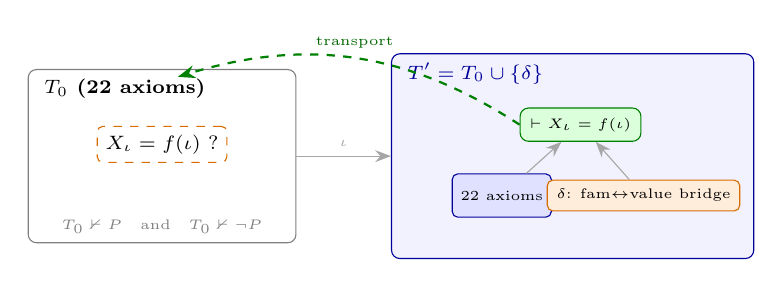
\begin{tikzpicture}[node distance=5mm and 8mm]
\node[draw=gray, rounded corners=3pt, minimum width=34mm, minimum height=22mm, font=\scriptsize] (T0) {};
\node[font=\scriptsize\bfseries, anchor=north west] at (T0.north west) {\;$T_0$ (22 axioms)};
\node[open, draw=orange!85!black, font=\scriptsize] at ($(T0.center)+(0,1.5mm)$) {$X_\iota = f(\iota)$ ?};
\node[font=\tiny, gray, anchor=south] at (T0.south) {$T_0 \nvdash P$ \; and \; $T_0 \nvdash \neg P$};
\node[draw=blue!60!black, fill=blue!5, rounded corners=3pt, minimum width=46mm, minimum height=26mm, right=12mm of T0, font=\scriptsize] (T1) {};
\node[font=\scriptsize\bfseries, anchor=north west, blue!60!black] at (T1.north west) {\;$T' = T_0 \cup \{\delta\}$};
\node[ax, font=\tiny] at ($(T1.center)+(-9mm,-5mm)$) (a22) {22 axioms};
\node[draw=orange!85!black, fill=orange!14, rounded corners=2pt, font=\tiny] at ($(T1.center)+(9mm,-5mm)$) (delta) {$\delta$: fam$\leftrightarrow$value bridge};
\node[goal, font=\tiny] at ($(T1.center)+(1mm,4mm)$) (iP) {$\vdash X_\iota = f(\iota)$};
\draw[fl] (a22) -- (iP); \draw[fl] (delta) -- (iP);
\draw[fl] (T0.east) -- node[above, font=\tiny] {$\iota$} (T1.west);
\draw[gl, dashed] (iP.west) to[bend right=25] node[above, font=\tiny, green!40!black] {transport} ($(T0.north)+(2mm,-1mm)$);
\end{tikzpicture}
\caption{The move that only a theory-as-data substrate permits. \textbf{How to read}:
each large rounded rectangle is a \emph{theory} (left, the reference $T_0$; right,
its extension $T'$); inside, blue boxes are axioms, the \textbf{orange} box the added
definition $\delta$ (and, at left, the orange hypothesis it answers), the green box
the goal now provable; the \textbf{dashed green arrow} is the transport of the result
back into $T_0$'s language. When a hypothesis is \emph{independent} (here the
family-value bridge, independent of $A_{T_0}$), no search closes it --- the only legal move extends the theory with a
definition $\delta$, proves the image, and transports the result back.}
\label{fig:extension}
\end{figure}

Read abstractly, the system is experimental inquiry in the zero-noise limit:
falsification is a derivation, theory revision is an executable operation with a
certified outcome, test severity is a mutation count, and the economy of measurement
is a budget with journaled overruns --- Popper, Lakatos, Mayo, and AGM as running
code rather than philosophy of science. That limit is what makes the corpus valuable
as training data: every label is exact.

The roadmap follows from the measurements. Replay instrumentation turns the existing
4{,}099-test corpus into $10^5$--$10^6$ certified (state, action, verdict) tuples
without formalizing a single new page --- the data factory is the same infrastructure
as the term cache that removes the dominant reconstruction cost. An environment API
($\mathit{reset}(T,P)$ / $\mathit{step}$) exposes the loop to any policy: frontier
models are rented and replaceable; the guidance memory $M(s)$ and its certified labels
are what accumulate and what no existing proof corpus provides. The twin detector's
second version reads the characterized term from the axiom's shape and covers the
parametric factories. And the strategic frontier is Bourbaki's Chapter~IV ---
structures and transport --- because that is where a theory created for one problem
learns to pay off in another.

A proof assistant certifies what we know. A certified failure corpus records how we
came to know it --- the walls, the repairs, the prices paid --- and for a machine that
must learn to \emph{create} theories rather than search within one, that is the
scarcer commodity.

\bibliographystyle{plain}
\bibliography{references}

\end{document}
